% Some LaTeX commands I define for my own nomenclature.
% If you have to, it's better to change nomenclature once here than in a 
% million places throughout your thesis!
\newcommand{\package}[1]{\textbf{#1}} % package names in bold text
\newcommand{\cmmd}[1]{\textbackslash\texttt{#1}} % command name in tt font 


%======================================================================
\chapter{Model Description}
%======================================================================

The model is composed of human population given by $N_{h}$ and
reservoir population given by $N_{r}$. We divide the human population ($N_{h}$) in $5$ categories namely, Susceptibles ($S_{h}$), Vaccinated ($V_{h}$), Exposed ($E_{h}$), Infected ($I_{h}$) and Recovered ($R_{h}$) whereas the reservoir population ($N_{r}$) is divided among Susceptibles ($S_{r}$), Infected($I_{r}$) and Recovered ($R_{r}$), such that
\[N_{h} = S_{h} + V_{h} + E_{h} + I_{h} + R_{h}\]
\[N_{r} = S_{r} + I_{r} + R_{r}\]

\begin{figure}[h]
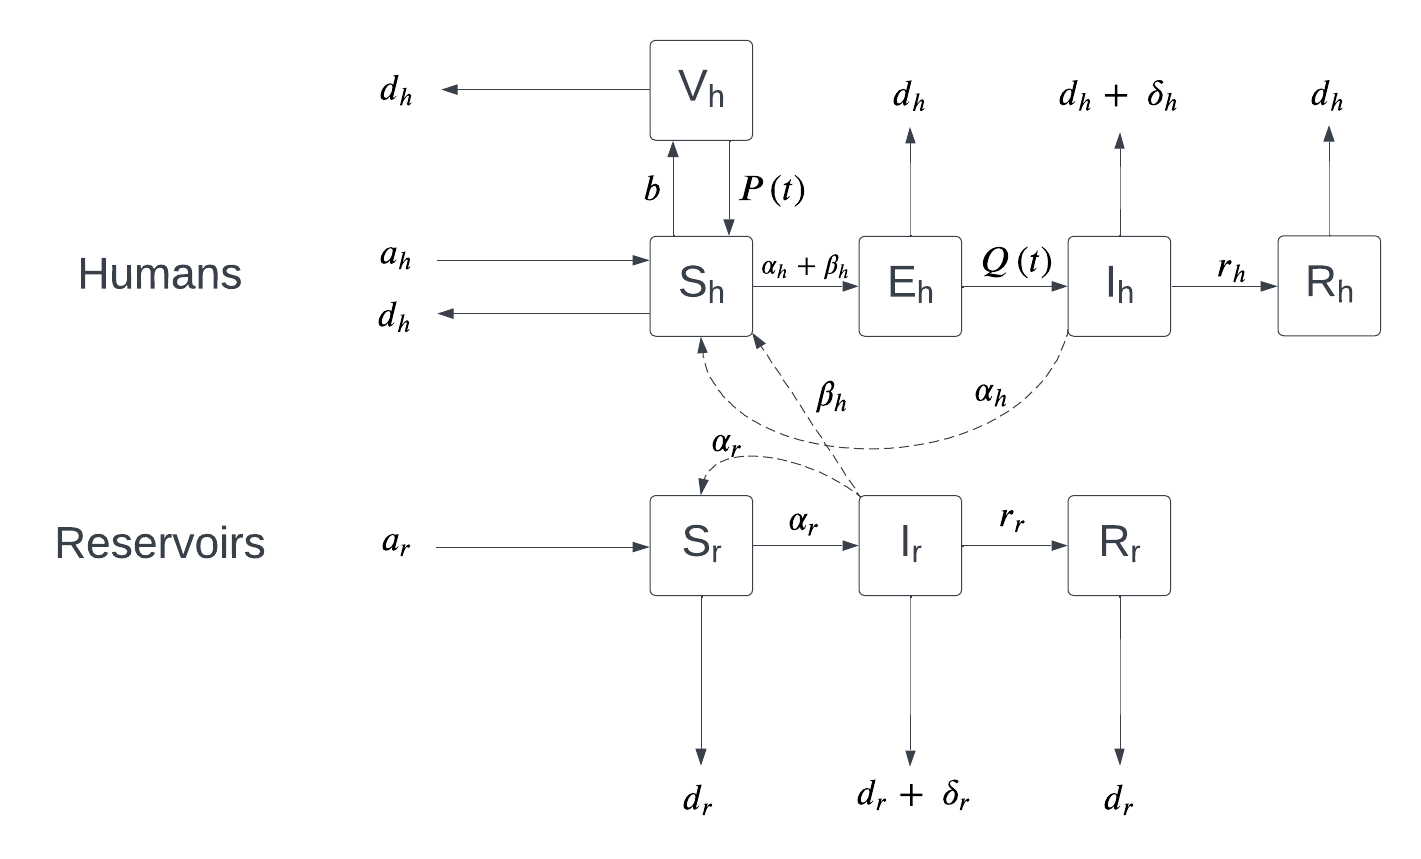
\includegraphics[width=\textwidth]{flow-diagram}
\caption{Model Flow Diagram}
\centering
\end{figure}
We assume that $a_{h}$ and $a_{r}$ is the constant birth rate of susceptible humans and reservoirs respectively and susceptibles are vaccinated at a constant rate $b$. $\alpha_{r}$, $\alpha_{h}$ and $\beta_{h}$ are the infection rates from reservoir to reservoir, reservoir to human and from human to human respectively.
To allow for a general latent period, we further assume that $P(t)$ is the probability of individuals remaining in the vaccinated class $t$ units after being vaccinated and $Q(t)$ is the probability of individuals remaining in the exposed class $t$ units after being exposed to the monkeypox virus. $r_{h}$ and $r_{r}$ are the recovery rates of the humans and the reservoirs respectively from the infection. Lastly, we consider that $d_{h}$ and $\delta_{h}$ is the natural and infection related death rate of humans whereas $d_{r}$ and $\delta_{r}$ is the natural and infection-related death rate of reservoirs.
According to the natural progression of the disease, we assume $P(t)$ and $Q(t)$ non-negative, non-increasing and piecewise continuous with 
\begin{center}
$P(0^{+}) = Q(0^{+}) = 1$ and $P(\infty) = Q(\infty) = 0$
\end{center}

The number of individuals who become exposed at some time $\mu \in (0,t)$ and are still in the exposed class at time $t$ is given by
\begin{equation}
E_{h}(t) = \int_{0}^{t} (\alpha_{h}S_{h}(\mu)I_{h}(\mu) +\beta_{h}S_{h}(\mu)I_{r}(\mu)) e^{-d_{h}(t-\mu)}Q(t-\mu) \,d\mu \label{exposed}
\end{equation}


and the number of individuals who get vaccinated at some time $\mu \in (0,t)$ and are still in the vaccinated class at time $t$ is given by
\begin{equation}
V_{h}(t) = \int_{0}^{t} bS_{h}(\mu)e^{-d_{h}(t-\mu)}P(t-\mu) \,d\mu \label{vaccinated}
\end{equation}


%Now, substituting $v = t-\mu$, we get

%\[E_{h}(t) = \int_{0}^{t} (\beta_{h}S_{h}(t-v)I_{h}(t-v) + \alpha_{h}S_{h}(t-v)I_{r}(t-v)) e^{-d_{h}v}Q(v) \,dv\]

%\[V_{h}(t) = \int_{0}^{t} bS_{h}(t-v)e^{-d_{h}(v)}P(v) \,dv\]
The general model is represented as follows
\begin{flalign} 
S_{h}'(t) &= a_{h}-d_{h}S_{h}(t)-bS_{h}(t)-(\alpha_{h}S_{h}(t)I_{h}(t)+\beta_{h}S_{h}(t)I_{r}(t))-\int_{0}^{t} bS_{h}(\mu)e^{-d_{h}(t-\mu)}P'(t-\mu) \,d\mu  \label{meq1}\\
%-------------------------------------------------------------
V_{h}'(t) &= bS_{h}(t)-d_{h}V_{h}(t)+\int_{0}^{t} bS_{h}(\mu)e^{-d_{h}(t-\mu)}P'(t-\mu) \,d\mu  \label{meq2}\\
%-------------------------------------------------------------
E_{h}'(t) &= \alpha_{h}S_{h}(t)I_{h}(t)+\beta_{h}S_{h}(t)I_{r}(t))-d_{h}E_{h}(t)+\int_{0}^{t} (\alpha_{h}S_{h}(\mu)I_{h}(\mu)+\beta_{h}S_{h}(\mu)I_{r}(\mu))e^{-d_{h}(t-\mu)}Q'(t-\mu) \,d\mu  \label{meq3}\\
%-------------------------------------------------------------
I_{h}'(t) &= -\int_{0}^{t} (\alpha_{h}S_{h}(\mu)I_{h}(\mu)+\beta_{h}S_{h}(\mu)I_{r}(\mu))e^{-d_{h}(t-\mu)}Q'(t-\mu) \,d\mu -d_{h}I_{h}(t) -\delta_{h}I_{h}(t) -r_{h}I_{h}(t)  \label{meq4}\\
%-------------------------------------------------------------
R_{h}'(t) &= r_{h}I_{h}(t) -d_{h}R_{h}(t) \label{meq5}\\ 
%-------------------------------------------------------------
S_{r}'(t) &= a_{r}-d_{r}S_{r}(t)-\alpha_{r}S_{r}(t)I_{r}(t)  \label{meq6}\\
%-------------------------------------------------------------
I_{r}'(t) &= \alpha_{r}S_{r}(t)I_{r}(t) -d_{r}I_{r}(t) -\delta_{r}I_{r}(t)- r_{r}I_{r}(t)  \label{meq7}\\
%-------------------------------------------------------------
R_{r}'(t) &= r_{r}I_{r}(t) -d_{r}R_{r}(t)  \label{meq8}
%-------------------------------------------------------------
\end{flalign}

To obtain more specific models, we have discussed four cases with different values for the functions $P(t)$ and $Q(t)$.

% CASE 1
Case \rom{1} [$P(t)=e^{-\omega t}, Q(t)=e^{-\omega t}$]

Equation \ref{exposed} becomes
\[E_{h}(t) = \int_{0}^{t} (\alpha_{h}S_{h}(\mu)I_{h}(\mu) + \beta_{h}S_{h}(\mu)I_{r}(\mu)) e^{(d_{h}+\omega)\mu-(d_{h}+\omega)t} \,d\mu\]
%-------------------------------------------------------------
\[\Rightarrow E_{h}(t) = e^{-(d_{h}+\omega)t}\int_{0}^{t} (\alpha_{h}S_{h}(\mu)I_{h}(\mu) + \beta_{h}S_{h}(\mu)I_{r}(\mu)) e^{(d_{h}+\omega)\mu} \,d\mu\]
%-------------------------------------------------------------
\[\Rightarrow E_{h}'(t) = -(d_{h}+\omega)E_{h}(t) + e^{-(d_{h}+\omega)t}(\alpha_{h}S_{h}(t)I_{h}(t) + \beta_{h}S_{h}(t)I_{r}(t)) e^{(d_{h}+\omega)t}\]
%-------------------------------------------------------------
\[\Rightarrow E_{h}'(t) = \alpha_{h}S_{h}(t)I_{h}(t) + \beta_{h}S_{h}(t)I_{r}(t)-(d_{h}+\omega)E_{h}(t)\]
%-------------------------------------------------------------
Again, equation \ref{vaccinated} becomes
\[V_{h}(t) = \int_{0}^{t} bS_{h}(\mu)e^{(d_{h}+\omega)\mu-(d_{h}+\omega)t} \,d\mu\]
%-------------------------------------------------------------
\[\Rightarrow V_{h}(t) = e^{-(d_{h}+\omega)t}\int_{0}^{t} bS_{h}(\mu) e^{(d_{h}+\omega)\mu} \,d\mu\]
%-------------------------------------------------------------
\[\Rightarrow V_{h}'(t) = -(d_{h}+\omega)V_{h}(t) + e^{-(d_{h}+\omega)t}bS_{h}(t) e^{(d_{h}+\omega)t}\]
%-------------------------------------------------------------
\[\Rightarrow V_{h}'(t) = bS_{h}(t)-(d_{h}+\omega)V_{h}(t)\]
%-------------------------------------------------------------
The model for case \rom{1} is represented as follows
\begin{flalign} 
S_{h}'(t) &= a_{h}+\omega V_{h}(t)-d_{h}S_{h}(t)-bS_{h}(t)-(\alpha_{h}S_{h}(t)I_{h}(t)+\beta_{h}S_{h}(t)I_{r}(t)) \label{case1meq1}\\
%-------------------------------------------------------------
V_{h}'(t) &= bS_{h}(t)-(d_{h}+\omega)V_{h}(t) \label{case1meq2}\\
%-------------------------------------------------------------
E_{h}'(t) &= \alpha_{h}S_{h}(t)I_{h}(t) + \beta_{h}S_{h}(t)I_{r}(t)-(d_{h}+\omega)E_{h}(t)  \label{case1meq3}\\
%-------------------------------------------------------------
I_{h}'(t) &= \omega E_{h}(t) -d_{h}I_{h}(t) -\delta_{h}I_{h}(t) -r_{h}I_{h}(t)  \label{case1meq4}\\
%-------------------------------------------------------------
R_{h}'(t) &= r_{h}I_{h}(t) -d_{h}R_{h}(t) \label{case1meq5}\\ 
%-------------------------------------------------------------
S_{r}'(t) &= a_{r}-d_{r}S_{r}(t)-\alpha_{r}S_{r}(t)I_{r}(t)  \label{case1meq6}\\
%-------------------------------------------------------------
I_{r}'(t) &= \alpha_{r}S_{r}(t)I_{r}(t) -d_{r}I_{r}(t) -\delta_{r}I_{r}(t)- r_{r}I_{r}(t)  \label{case1meq7}\\
%-------------------------------------------------------------
R_{r}'(t) &= r_{r}I_{r}(t) -d_{r}R_{r}(t)  \label{case1meq8}
%-------------------------------------------------------------
\end{flalign}